\section{Eksperymenty}
\subsection{Klasyfikacja kNN przy podziale zbioru 80:20}
W przeprowadzonym eksperymencie dokonano podziału zbioru 80:20 (20 procent danych testowych). Następnie zdefiniowano klasyfikator z parametrem n\_neighbors równym 5. Kolejnym krokiem było wytrenowanie klasyfikatora i przeprowadzenie predykcji na zbiorze testowym:\\

\begin{lstlisting}[language=Python, caption=Definicja i uzycie kNN]
from sklearn.neighbors import KNeighborsClassifier
from sklearn import metrics

knn = KNeighborsClassifier(n_neighbors=5)
knn.fit(X_train, y_train)

y_pred = knn.predict(X_test)
\end{lstlisting}

\subsubsection{Wyniki}
Podstawowe metryki dla pierwszego eksperymentu wynosiły precyzja (\textit{Precision}): 0.85 a dokładność (\textit{Accuracy}): 0.7875. Co nie stanowi wiele informacji, korzystam więc z gotowych metryk dostępnych w bibliotece scikit-learn:\\

\begin{verbatim}
                             precision  recall f1-score support

            Basilar-type aura     1.00    0.29     0.44       7
 Familial hemiplegic migraine     0.50    0.80     0.62       5
        Migraine without aura     0.62    0.62     0.62       8
                        Other     1.00    0.67     0.80       3
 Sporadic hemiplegic migraine     0.00    0.00     0.00       4
   Typical aura with migraine     0.82    0.94     0.88      49
Typical aura without migraine     1.00    1.00     1.00       4

                     accuracy                      0.79      80
                    macro avg     0.71    0.62     0.62      80
                 weighted avg     0.77    0.79     0.76      80
\end{verbatim}

Jak widzimy na powyższym listingu (i o czym również informuje nas warning biblioteki scikit-learn) klasa Sporadic hemiplegic migraine nie wystąpiła w zbiorze testowym ani razu. Zbiór nie jest ani specjalnie liczny ani tez zbalansowany wiec sytuacja taka jest jest zaskoczeniem ale nie przestaje to podważać efektywności walidacji naszych badań. W kolejnym eksperymencie przedstawiam za to inne proporcje podziały zbioru.

\subsection{Klasyfikacja kNN przy podziale zbioru 75:25}
Przebieg eksperymentu był dokładnie taki sam jak w poprzednim z tym że podział zbioru na dane uczące i testowe dokonał się w proporcjach 75:25 (tak jak poprzednio ze sztuczną losowością aby zapewnić powtarzalność wyników).\\

\subsubsection{Wyniki}
Zmiana podziału zbioru nie wpłynęła zasadniczo na wartość precyzji i dokładności ale nie istniał juz problem braku klas w zbiorze testowym, co nie przekreśla juz sensowności przeprowadzonych obliczeń. Nadal jednak zaden z obiektów klasy "Sporadic hemiplegic migraine" nie został poprawnie rozpoznany co dalej, dla tego podzbioru klas zarówno precyzje jak i recall równe zero.\\

\begin{verbatim}
                            precision  recall f1-score support

            Basilar-type aura    1.00    0.12     0.22       8
 Familial hemiplegic migraine    0.57    0.80     0.67       5
        Migraine without aura    0.64    0.64     0.64      11
                        Other    1.00    0.50     0.67       4
 Sporadic hemiplegic migraine    0.00    0.00     0.00       5
   Typical aura with migraine    0.77    0.94     0.85      62
Typical aura without migraine    1.00    0.60     0.75       5

                     accuracy                     0.75     100
                    macro avg    0.71    0.51     0.54     100
                 weighted avg    0.75    0.75     0.71     100
\end{verbatim}

Ogólna wartość precyzji (\textit{Precision}) dla całego zbioru testowego pozostała na poziomie 85\%. Dokładność ($Accuracy$) na zbioru testowego spadła o 3,75 punktu procentowego (do poziomu 75\%).\\

W przypadku walidacji krzyzowej precyzja wahała się pomiędzy 57 a 100\% (w stosunku do poprzedniego podziału nieznaczne wzrosty w przypadku mniej licznych klas). Recall charakteryzował się duzym rozrzutem wartości - mniej liczne klasy miały recall niekiedy i 0-12\% a te bardziej liczne 80-90\%.\\

Średnia wartość recallu to 51\% a średnia wazona 75\% (ta właśnie uwzględniała nierówną liczebność klas). Podobna różnica miała miejsce w przypadku precyzji wyliczonej przy zastosowaniu walidacji krzyzowej - średnia wartość 71\% - średnia wazona 75\%.\\

\subsection{Klasyfikacja Naiwnym Klasyfikatorem Bayesa}
W eksperymencie tym sprawdziłem wyniki klasyfikacji Naiwnym Klasyfikatorem Bayesa. Biblioteka scikit-learn umozliwia przeprowadzenie tzn \textit{Categorical Classication (Categorical Naive Bayes)} gdzie w przeciwieństwie do popularnej klasyfikacji binarnej, metoda jest w stanie zwrócić dwie informacje: etykietę klasy będącej wynikiem klasyfikacji oraz listę ze stopniami podobieństwa dla wszystkich klas.\\

\begin{lstlisting}[language=Python, caption=Definicja i uzycie CategoricalNB]
from sklearn.naive_bayes import CategoricalNB

gnb = CategoricalNB()
    
y_pred = gnb.fit(X_train, y_train).predict(X_test)
\end{lstlisting}    

\subsubsection{Wyniki}
O ile wyniki dokładności (\textit{Accuracy}) wyglądały podobnie niz dla np. kNN - dokładnie 75\%. O tyle wyniki dla całości zbiory prezentowały się gorzej o 5-6 punktów procentowych niz dla kNN - precyzja średnia 64\% (względem 71\%) oraz precyzja wazona 69\% (względem 75\%). Wyniki dla poszczególnych klas dla precyzji potrafiły się różnić o 20-30 punktów procentowych względem kNN nie dając wyraźniej korelacji względem liczebności klas. Wyniki dla recall po trafiły być niekiedy diametralnie różne - 88\%-12\% a niekiedy znikomo - 92\%-94\% względem kNN.\\

\begin{verbatim}
                              precision  recall  f1-score   support

            Basilar-type aura      1.00    0.88      0.93         8
 Familial hemiplegic migraine      0.75    0.60      0.67         5
        Migraine without aura      0.29    0.18      0.22        11
                        Other      1.00    1.00      1.00         4
 Sporadic hemiplegic migraine      0.00    0.00      0.00         5
   Typical aura with migraine      0.76    0.92      0.83        62
Typical aura without migraine      0.67    0.40      0.50         5

                     accuracy                        0.75       100
                    macro avg      0.64    0.57      0.59       100
                 weighted avg      0.69    0.75      0.71       100
\end{verbatim}

Niezwykle istotną możliwością wykorzystania Naiwnego Klasyfikatora Bayesa było wyświetlenie podobieństwa testowanej klasy względem wszystkich klas.\\

Niektóre z klas (niekoniecznie te bardziej licznie) przedstawiały bardzo jednoznaczną klasyfikację, np:\\

\begin{verbatim}
    Other
    0.0009411289994916489: 	 Basilar-type aura
    0.00024106562936048384:  Familial hemiplegic migraine
    1.3757510137960067e-06:  Migraine without aura
    0.9987800638900048:      Other
    5.212399025390643e-06: 	 Sporadic hemiplegic migraine
    3.406207926665455e-08: 	 Typical aura with migraine
    3.111926902521578e-05: 	 Typical aura without migraine
\end{verbatim}

dla innych (często dla konkretnych jak np. Typical aura without migraine czy Migraine without aura) mieliśmy rozkłady bardzo zróżnicowane:

\begin{verbatim}
    Typical aura without migraine
    0.08048228203931468:    Basilar-type aura
    0.2633221828713967:     Familial hemiplegic migraine
    0.0009416760319083586:  Migraine without aura
    0.005682255909626338:   Other
    0.22367861315019222:    Sporadic hemiplegic migraine
    0.15361555787258202:    Typical aura with migraine
    0.2722774321249797:     Typical aura without migraine
\end{verbatim}
albo nawet niemal bilateralne:

\begin{verbatim}
    Migraine without aura
    0.000315062484758524:    Basilar-type aura
    0.0008466488192796888:   Familial hemiplegic migraine
    0.516090617842986:       Migraine without aura
    0.001079067159295874:    Other
    0.0038615304383266213:   Sporadic hemiplegic migraine
    0.4772101808065339:      Typical aura with migraine
    0.0005968924488194133:   Typical aura without migraine
\end{verbatim}

\subsection{Selekcja i ekstrakcja cech}
W czasie wykonanych eksperymentów wykorzystano dwa sposoby selekcji cech: SKB i RFE, oraz mechanizm wyodrębnienia cech PCA.\\

Definicja algorytmu selekcji cech SKB (czyli Select k Best), wybór k dziesięciu najlepszych i wyświetlenie nowych nazw cech:
\begin{lstlisting}[language=Python, caption=Definicja selektora SKB]
from sklearn.feature_selection import SelectKBest, chi2

skb = SelectKBest(chi2, k = 10)
X2 = skb.fit_transform(X, y)
\end{lstlisting}

Definicja selektora cech RFE (dla klasyfikatora SVC i redukcji do 10 cech):

\begin{lstlisting}[language=Python, caption=Definicja selektora RFE]
from sklearn.feature_selection import RFE

svc = SVC(kernel = 'linear')

rfe = RFE(estimator = svc, n_features_to_select = 10, step = 1)
X3 = rfe.fit_transform(X, y.values.ravel())
\end{lstlisting}

Definicja ekstraktora cech PCA (ekstrakcja do 4 cech).

\begin{lstlisting}[language=Python, caption=Definicja ekstraktora cech PCA]
from sklearn.decomposition import PCA

pca = PCA(n_components = 4)
X4 = pca.fit_transform(X)
\end{lstlisting}

\subsubsection{Wyniki}
Wyniki prezentowały się następująco:

\begin{verbatim}
Średnia dokładność klasyfikacji z wykorzystaniem klasyfikatora ...

    kNN wyniosła:                0.8024999999999999
    kNN i metody SKB wyniosła:   0.7825
    kNN i metody RFE wyniosła:   0.865
    kNN i metody PCA:            0.7

    SVC wyniosła:                0.8825
    SVC i metody SKB wyniosła:   0.8
    SVC i metody RFE wyniosła:   0.8825
    SVC i metody PCA:            0.735
\end{verbatim}

Co interesujące to właśnie dyskusyjny eksperyment klasyfikacji KNN z selekcją RFE poprawił wynik dla kNN o 8 punktów procentowych a np. SKB pogorszył go o dwa. W przypadku klasyfikatora SVC w/w metody albo nie zmieniły wyniku (RFE) albo pogorszyły wynik od 8-10 punktów procentowych.\\

Uzyty zbiór nie był zbiorem licznym ani tez obliczenia na nim wykonywane nie wymagały duzych mocy obliczeniowych. Nie istniało zatem zadne uzasadnienie stosowania którejkolwiek z w/w metod poniewaz przy praktycznie zerowej optymalizacji otrzymywaliśmy gorsze wyniki.\\

\subsection{Perceptron wielowarstwowy}
Kolejnym z przeprowadzonych eksperymentów było użycie perceptronu wielowarstwowego. Podział zbioru to 75\% na dane treningowe i 25\% na dane testowe. Ponownie wykorzystaliśmy bibliotekę scikit-learn:

\begin{lstlisting}[language=Python, caption=Definicja perceptronu wielowarstwowego]
    from sklearn.neural_network import MLPClassifier
    mlp = MLPClassifier(hidden_layer_sizes=(6),
                         max_iter=50000, 
                         alpha=0.0001,
                         solver='adam',
                         activation= 'logistic', 
                         random_state=25,
                         tol=0.0000001)
\end{lstlisting}

Wyjaśnienie wykorzystanych parametrów:
\begin{enumerate}
    \item hidden\_layer\_sizes - ilość warstw ukrytych
    \item max\_iter - liczba epok
    \item alpha - współczynnik regularyzacji który zapobiega zjawisku przeuczenia
    \item solver - wybór algorytmu optymalizacji "adam".
    \item activation - wybór sigmoidalnej funkcji aktywacji
    \item random\_state - ziarno generatora liczb losowych
    \item tol - tolerancja dla kryterium stop. Algorytm zatrzymuje się, jeśli zmiana wyniku (kosztu) jest mniejsza niż ta wartość.
\end{enumerate}

\subsubsection{Wyniki}
Wyniki działania perceptronu okazały się zaskakująco dobre. Przy relatywnie niskiej ilości warstw ukrytych (6), przeciętnej ilości epok (50000) i popularnym optymalizatorze ("adam") osiągnęliśmy dokładność (Accuracy) na poziomie 94\% i średnią ważoną precyzję 95\%. Recall wahał się od 60\% do 100\% (przy średniej wazonej wartości 94\%) a współczynnik F1 od 75\% do 100\% (przy średniej ważonej wartości 93\%).\\
\begin{verbatim}
                              precision  recall f1-score  support

            Basilar-type aura      1.00    0.20     0.33        5
 Familial hemiplegic migraine      0.57    0.80     0.67        5
        Migraine without aura      1.00    1.00     1.00       12
                        Other      1.00    1.00     1.00        3
 Sporadic hemiplegic migraine      0.75    1.00     0.86        3
   Typical aura with migraine      0.97    0.99     0.98       67
Typical aura without migraine      1.00    1.00     1.00        5

                     accuracy                       0.94      100
                    macro avg      0.90    0.86     0.83      100
                 weighted avg      0.95    0.94     0.93      100

NN Accuracy =  0.94
\end{verbatim}

Przy mniejszej ilości epok (5000) takiej samej ilości warstw ukrytych (6) i tym samym optymalizatorze ("adam") osiągnęliśmy dokładność (Accuracy) na poziomie 96\% i średnią ważoną precyzję 97\%. Recall wahał się od 60\% do 100\% a współczynnik F1 od 75\% do 100\% (przy średniej wazonej wartości 96\%) z tym że biblioteka wyświetliła ostrzeżenie że optymalizator nie zakończył działania więc wyniki mogę byś nieoptymalne.\\

\begin{verbatim}
                              precision  recall f1-score  support

            Basilar-type aura      1.00    0.60     0.75        5
 Familial hemiplegic migraine      0.67    0.80     0.73        5
        Migraine without aura      1.00    1.00     1.00       12
                        Other      1.00    1.00     1.00        3
 Sporadic hemiplegic migraine      0.75    1.00     0.86        3
   Typical aura with migraine      0.99    0.99     0.99       67
Typical aura without migraine      1.00    1.00     1.00        5

                     accuracy                       0.96      100
                    macro avg      0.91    0.91     0.90      100
                 weighted avg      0.97    0.96     0.96      100

NN Accuracy =  0.96
\end{verbatim}

\subsection{Sieć głęboka z funkcją aktywacji Softmax}
Perceptron wielowarstwowy choć dawał świetne wyniki to jednak dawał wynik przynależności do najbardziej prawdopodobnej klasy. W zagadnieniu klasyfikacji bólów głowy interesującym byłoby pokazać wynik w postać stopnia podobieństwa przynależności do każdej z mozliwych klas. Z pomocą przychodzi nam funkcja aktywacji Softmax i możliwość zastosowania jej w głębokich sieciach neuronowych.\\

W przypadku funkcji aktywacji Softmax konieczne jest uzycie enkodera etykiet klas - czy zamianę etykiet na przyporządkowane im liczby. Następnie w/w liczby zamieniamy na tzw. format hot-one czyli format gdzie danej liczbie przyporządkowujemy ciąg binarny zer oraz jednej jedynki w miejscu w szeregu odpowiadającym danej liczbie. Po testowej klasyfikacji musimy nasze wyniki zdekodować z powrotem do formatu etykiet. Wszystkie te operacje umozliwia nam biblioteka scikit-learn.\\

Do definicji sieci głębokiej uzywam biblioteki TensorFlow i jej części Keras.
\begin{lstlisting}[language=Python, caption=Definicja sieci głębokiej z funkcją aktywacji Softmax]
model=tf.keras.models.Sequential()
model.add(tf.keras.layers.Dense(64, activation='relu'))
model.add(tf.keras.layers.Dense(32, activation='relu'))
model.add(tf.keras.layers.Dense(num_classes, 
                                activation='softmax'))
model.build(input_shape=23)
model.compile(optimizer='Adam',
              loss='categorical_crossentropy',
              metrics=['accuracy'])
\end{lstlisting}

W powyższej definicji mamy:
\begin{enumerate}
    \item definicje modelu sekwencyjnego
    \item definicje warstwy gęstej (Dense, wszystkie neurony połączone) z 64 neuronami i funkcją aktywacji ReLU.
    \item definicje warstwy gęstej (Dense, wszystkie neurony połączone) z 32 neuronami i funkcją aktywacji ReLU. 
    \item definicje warstwy gęstej (Dense) z funkcją aktywacji Softmax.
    \item określenie ilości wejść - 23 bo tyle mamy cech.
    \item kompilację modelu z optymalizatorem "adam", określeniem funkcji straty "categorical\_crossentropy" i definicje metryk.
\end{enumerate}


Następnie rozpoczynam trenowanie modelu dla 50 epok, wydzielenie 20\% zbioru testowego na zbiór walidacyjny i zapis modelu:
\begin{lstlisting}[language=Python, caption=Definicja sieci głębokiej z funkcją aktywacji Softmax]
history = model.fit(X_train,
                    y_train_one_hot,
                    epochs=50,
                    verbose=1,
                    validation_split=0.2)
tf.keras.models.save_model(model,'../models/softmax.keras')
\end{lstlisting}


Wyświetlenie wykresu wartości funkcji straty i porównanie jej z wartością straty na zbioru walidacyjnego daje mi orientacyjną możliwość oceny słuszności doboru ilości epok.\\


\begin{figure}[h]
    \centering
    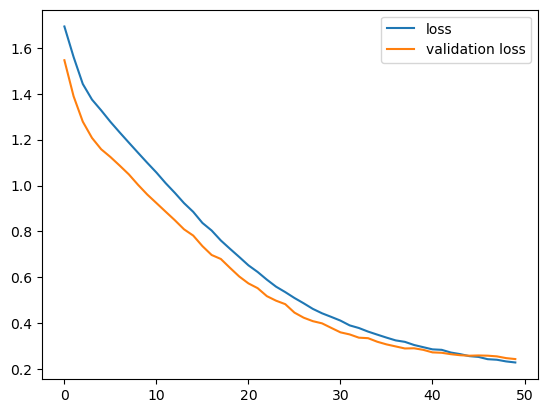
\includegraphics[scale=0.8]{valloss}
    \caption{Wykresy funkcji strat}
    \label{fig:valloss}
\end{figure}

\subsubsection{Wyniki}
Dla zbioru testowego osiągnęliśmy 95\% dokładność.\\

\begin{verbatim}
4/4 ==================== 0s 801us/step - accuracy: 0.9446 - loss: 0.2267
    Loss: 0.21024955809116364, Accuracy: 0.949999988079071
\end{verbatim}

Najciekawszym aspektem wykorzystania funkcji Softmax jest możliwość wyświetlenia podobieństwa do wszystkich możliwych klas. Oto kilka przykładów dla konkretnych przypadków, co zrobiłem na dwa sposoby. Pierwszy z nich wyświetlał wszystkie klasy i podobieństwa konkretnego przypadków do każdej z nich:\\

\begin{verbatim}
    Class: Basilar-type aura,             Probability: 0.25
    Class: Familial hemiplegic migraine,  Probability: 0.63
    Class: Migraine without aura,         Probability: 0.00
    Class: Other,                         Probability: 0.09
    Class: Sporadic hemiplegic migraine,  Probability: 0.03
    Class: Typical aura with migraine,    Probability: 0.00
    Class: Typical aura without migraine, Probability: 0.00
\end{verbatim}

a drugi z nich wyświetlał tabelę: enkodowana etykieta klasy, pełna etykieta klasy i prawdopodobieństwo do danej klasy analizowanego przypadku. Wartości uszeregowane malejąco wg podobieństwa:

\begin{verbatim}
                                Type  Probabilities
    1   Familial hemiplegic migraine           0.63
    0              Basilar-type aura           0.25
    3                          Other           0.09
    4   Sporadic hemiplegic migraine           0.03
    5     Typical aura with migraine           0.00
    6  Typical aura without migraine           0.00
    2          Migraine without aura           0.00
\end{verbatim}